\chapter{Lieu de stage}

\section{University of Westminster}

\subsection{Pr\'esentation}

\parpic{
	\begin{minipage}{0.27\textwidth}
		
\includegraphics[scale=1.0]{westminsterBlason.jpg}
		\captionof{figure}{Blason de l'Universit\'e}
	\end{minipage}}
L'Universit\'e de Westminster est une universit\'e publique de recherche situ\'ee \`a Londres. 
\`A sa fondation, en 1838, elle portait le nom de \textit{Royal Polytechnic Institution} et \'etait la premi\`ere \'ecole polytechnique ouverte en Angleterre.
Son but \'etait de fournir une institution o\`u le public peut, \`a moindre co\^ut, acqu\'erir une connaissance pratique des divers arts et branches de la science en rapport avec les fabricants industriels, les op\'erations mini\`eres et l'\'economie rurale.
Sa fondation est une r\'eaction \`a la popularit\'e grandissante de l'enseignement de type polytechnique en Europe continentale. 
Notamment avec l'Allemagne et la \textit{Fachhochschule}, la France et l'\textit{\'Ecole Polytechnique} ou encore les \'Etats-Unis et la \textit{Rensselaer Polytechnic Institute}.

En 1970, la \textit{Royal Polytechnic Institution} devient \textit{Polytechnic of Central London} apr\`es avoir fusionn\'e avec \textit{Holborn College of Law, Languages and Commerce}.
C'est en 1992 que le statut d'universit\'e fut attribu\'e \`a Westminster qui devint \textit{University of Westminster}.

\subsection{Les diff\'erents campus et \'ecoles}
\label{section:campus}

L'Universit\'e compte quatre principaux campus, trois dans le centre de Londres : Regent, Cavendish, Marylebone et le quatri\`eme \`a Harrow, \`a l'ouest de Londres.

\begin{itemize}
	\item \textbf{Regent} : situ\'e au 309 Regent Street, c'est le campus le plus ancien de l'Universit\'e, il contient une \'ecole : 
		\textit{School of Social Sciences, Humanities and Languages};

	\item \textbf{Cavendish} : situ\'e au 101-115 New Cavendish Street, dans le quartier de Fitzrovia proche de West End de Londres (entre Marylebone, BloomsBury et au nord de Soho), ce campus contient trois \'ecoles : 
		\textit{School of Electronics and Computer Science}, \textit{School of Life Sciences} et \textit{Westminster Exchange} dont le but principal est l'am\'elioration de l'\'education;

	\item \textbf{Marylebone} : situ\'e sur Marylebone Road, en face du c\'el\`ebre mus\'ee de cire \textit{Madame Tussauds}, il contient deux \'ecoles :
		\textit{School of Architecture and the Built Environment} et \textit{Westminster Business School};

	\item \textbf{Harrow} : situ\'e dans le village de style victorien Harrow-on-the-Hill surplombant Londres, ce campus contient une \'ecole : 
		\textit{School of Media, Art and Design}.

\end{itemize}

\begin{figure}[!ht]
	\centering
	\subfloat[Fa\c{c}ade]{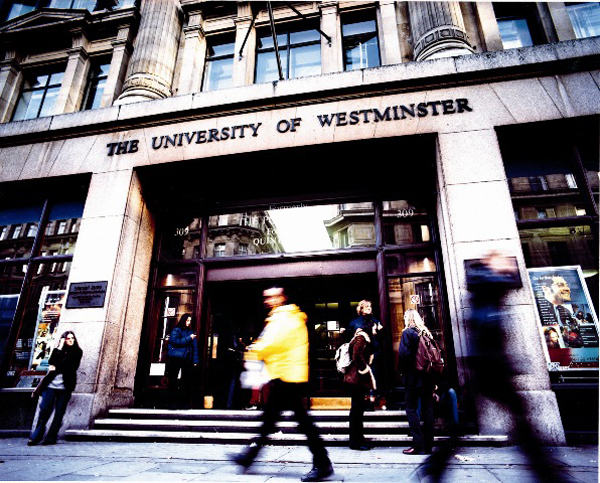
\includegraphics[scale=0.3]{westminsterRegentExterieur.jpg}}
	\qquad
	\subfloat[Entr\'ee]{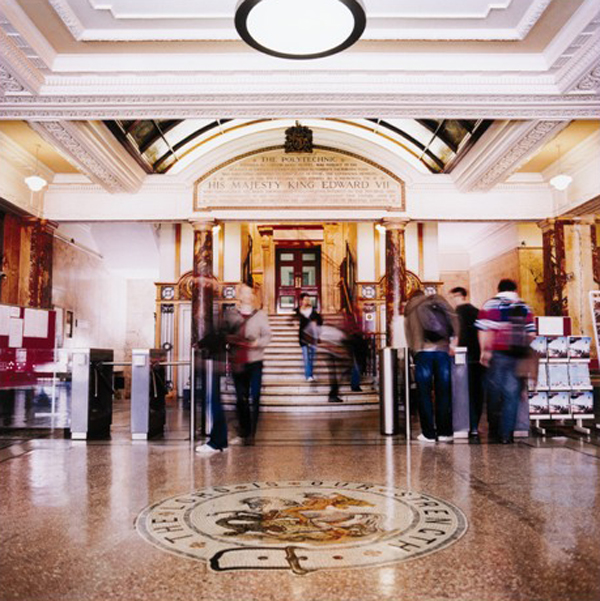
\includegraphics[scale=0.242]{westminsterRegentInterieur.jpg}}
	\caption{Campus de Regent Street}

\end{figure}

\noindent Outre ces principaux campus, l'Universit\'e compte deux autres sites : 

\begin{itemize}
	\item \textbf{Little Tichtfield Street} : situ\'e au 4-12 Little Titchfield street, il contient une \'ecole : 
		\textit{School of Law};
	\item \textbf{Wells Street} : situ\'e au 32-38 Wells street, juste au coin des autres b\^atiments du campus de Regent, il offre une grande vari\'et\'e de salles de classe.

\end{itemize}

\vspace{0.20cm}

L'Universit\'e g\`ere \'egalement le \textit{Westminster International University} \`a Tachkent en Ouzb\'ekistan ainsi qu'un campus satellite \`a Paris \`a travers l'Acad\'emie Diplomatique de Londres.

\subsection{Quelques informations sur l'Universit\'e}

L'Universit\'e se situe officiellement au 309 Regent Street London W1B 2HM.
Elle compte en 2011 plus de 20 000 \'etudiants venant de plus de 150 nations diff\'erentes gr\^ace \`a de nombreux programmes d'\'echange avec d'autres universit\'es.

\noindent Parmi ses dipl\^om\'es les plus prestigieux :

\begin{itemize}
	\item Sir \textbf{Alexander Fleming}, biologiste et pharmacologue britannique, prix Nobel de Physiologie ou M\'ed\'ecine en 1945 avec Ernst Boris Chain et Sir Howard Walter Florey pour la d\'ecouverte de la p\'enicilline et de son effet curatif sur diverses maladies infectieuses;
	\item \textbf{Christopher Bailey}, directeur de la cr\'eation chez \textit{Burberry};
	\item \textbf{Charlie Watts}, musicien et batteur des \textit{Rolling Stones}.

\end{itemize}

\vspace{0.20cm}

\noindent Concernant les cours, l'Universit\'e donne acc\`es \`a plus de 300 cours diff\'erents.

\section{School of Electronics and Computer Science}

Le stage s'est d\'eroul\'e dans cette \'ecole se trouvant, comme vu au \S~\ref{section:campus}, dans le campus Cavendish au 101-115 New Cavendish Street. 
La figure~\ref{figure:westminsterNewCavendish} montre une vue ext\'erieure du b\^atiment avec la BT Tower, tour de communication poss\'ed\'ee par l'op\'erateur de t\'el\'ecommunications BT Group, se trouvant juste \`a c\^ot\'e.

\begin{figure}[!ht]
	\centering
	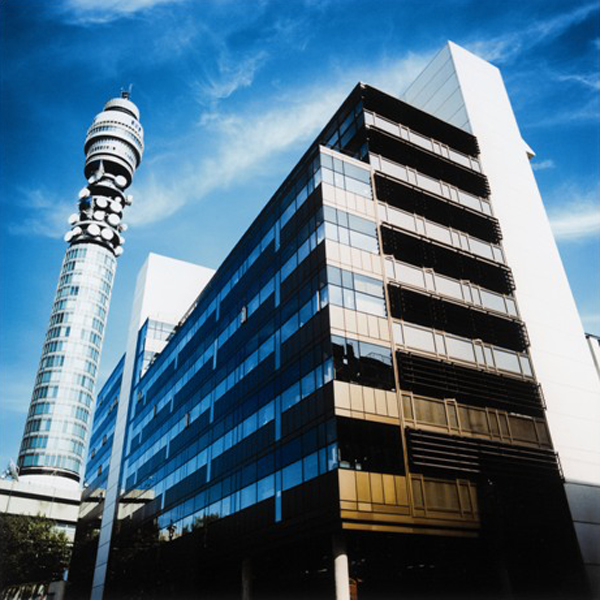
\includegraphics[scale=0.242]{westminsterNewCavendish.jpg}
	\caption{Campus de New Cavendish Street}
	\label{figure:westminsterNewCavendish}

\end{figure}

L'\'ecole propose divers parcours, aussi bien dans le domaine de la recherche que dans celui des \'etudes, allant de l'ing\'enierie \'electronique et informatique, aux math\'ematiques appliqu\'ees.
Ainsi de nombreuses mati\`eres peuvent \^etre abord\'ees dans la formation comme la gestion des syst\`emes d'informations, la programmation parall\`ele et distribu\'ee, l'intelligence artificielle mais aussi le d\'eveloppement de jeux vid\'eos et bien d'autres.

\noindent Il existe quatre grands p\^oles de recherche au sein de l'\'ecole qui sont :

\textit{Electronic and Communication Engineering}, qui se concentre sur le traitement de signaux ainsi que dans la conception de composants et circuits pour les syst\`emes de communication;

\textit{Operational Research and Intelligent Systems}, dont les activit\'es sont principalement la mod\'elisation quantitative des syst\`emes complexes pour soutenir des processus d\'ecisionnels, la gestion des donn\'ees et des informations, les technologies de bases de donn\'ees destin\'ees au processus de gestion et d'interop\'erabilit\'e dans les environnements o\`u les logiciels sont omnipr\'esents;

\textit{Parallel and Distributed Computing}, qui s'int\'eresse \`a la recherche et au d\'eveloppement dans le domaine des calculs parall\`eles et distribu\'es;

\textit{Semantic Computing and Systems Engineering}, regroupe des chercheurs de diff\'erentes disciplines, comme le g\'enie logiciel, les interactions homme-machine, et aborde les aspects th\'eoriques et pratiques de l'informatique s\'emantique.

\section{\'Equipes int\'egr\'ees}

Le projet {\YuukouII} -- sur lequel j'ai travaill\'e pendant mon stage -- regroupe deux services de l'Universit\'e. 
D'une part l'\textit{Infrastructure Team}, et d'autre part l'\textit{Information Systems and Library Services} (ISLS).
Le but de mon stage \'etant de fournir un pilote de ce qu'il est possible de faire afin que mon travail puisse \^etre repris par les deux services et d\'evelopp\'e plus en profondeur.

\subsection{\textit{Infrastructure Team}}

L'\textit{Infrastructure Team} est une \'equipe de 13 personnes dans la \textit{School of Electronics and Computer Science} qui a pour r\^ole de g\'erer les laboratoires sp\'ecialis\'es de l'\'ecole.
Ce sont 34 laboratoires de l'\'ecole qui sont sous la responsabilit\'e de cette \'equipe.
Ces laboratoires sont dit sp\'ecialis\'es du fait des possibilit\'es qui peuvent y \^etre r\'ealis\'ees : l'installation de nouveaux syst\`emes d'exploitations sur les ordinateurs par exemple.

L'\'equipe apporte aussi un support pour les laboratoires d'enseignement et pour les groupes de recherches dans l'\'ecole.
Elle reprend et \'etend les services fournis par les services centraux informatiques (voir ISLS au \S~\ref{section:ISLS}) comme l'authentification, les quotas de disques, le r\'eseau ou encore les outils d'enseignement.

\subsection{\textit{Information Systems and Library Services}}
\label{section:ISLS}

ISLS est un d\'epartement dont le but est de contribuer \`a la qualit\'e de l'\'education dans l'Universit\'e de Westminster \`a travers le d\'eveloppement et la livraison de services.

\noindent Le d\'epartement est compos\'e de cinq services qui sont :

\begin{itemize}
	\item \textit{Archive Services}, qui g\`ere les archives de l'Universit\'e;
	\item \textit{Corporate Information}, qui d\'eveloppe et livre des applications qui prennent en charge le fonctionnement des activit\'es (enregistrement des \'etudiants, emplois du temps, \ldots);
	\item \textit{Infrastructure}, qui g\`ere l'infrastructure informatique pour fournir des services informatiques et de t\'el\'ecommunications;
	\item \textit{Learning and Research Support}, qui g\`ere la biblioth\`eque et les services informatiques pour le personnel et les \'etudiants;
	\item \textit{Resources and Planning}, qui g\`ere les ressources et le planning du d\'epartement.

\end{itemize}

\section{\textit{Centre for Parallel Computing}}

Durant toute la dur\'ee de mon stage, j'ai travaill\'e dans le \textit{Centre for Parallel Computing} (CPC).
Le bureau se situe au 7\textsuperscript{e} \'etage de la \textit{School of Electronics and Computer Science} et est compos\'e de sept personnes.
Cette \'equipe appartient au p\^ole recherche \textit{Parallel and Distribued Computing}.

Ce centre se concentre sur la recherche dans la technologie et les applications de calculs parall\`eles et distribu\'es.
Les activit\'es du centre incluent le d\'eveloppement d'outils et d'environnements pour soutenir le cycle de vie dans le g\'enie logiciel comme la simulation d'\'ev\`enements discrets en parall\`ele.
Les chercheurs travaillent en collaboration avec l'Universit\'e hongroise Sztaki.

\noindent Parmi les projets d\'evelopp\'es par le service, on peut citer :

\begin{itemize}
	\item \textbf{Gemlca} (\textit{Grid Execution Management for Legacy Code Applications}), solution g\'en\'erale dont le but est de deployer le code d'applications existantes, quelque soit le langage, comme un service de grille;
	\item \textbf{NGS} (\textit{National Grid Service}), solution dont le but est de fournir un acc\`es \'electronique coh\'erent pour les chercheurs du Royaume-Uni \`a toutes les ressources de calculs et de donn\'ees ainsi qu'\`a l'\'equipement n\'ecessaire pour mener \`a bien leurs travaux, ind\'ependamment de l'emplacement de la ressource ou du chercheur;
	\item \textbf{SHIWA} (\textit{SHaring Interoperable Workflows for lages-scale scientific simulations on Available DCIs}\protect\footnote{\textit{Distributed Computing Infrastructure}}), projet qui a pour but l'interop\'erabilit\'e de diff\'erents syst\`emes de \textit{workflow}$^*$ europ\'een (comme Moteur, P-Grade, Askalon ou Gwes) \`a l'aide de l'approche par granularit\'e (grain fin ou grossier).

\end{itemize}

\vspace{0.20cm}

Pendant le stage, j'ai \'et\'e rejoint par deux \'etudiants en troisi\`eme ann\'ee de licence informatique \`a l'Universit\'e de Franche-Comt\'e de Besan\c{c}on : Yacine MAGHEZZI, travaillant sur la partie affichage du projet qui m'a \'et\'e confi\'e (plus d'explications au \S~\ref{section:architectureProjet}) et Damien HOSTACHE, travaillant sur le d\'eveloppement d'une application pour le portail Web de l'Universit\'e de Westminster dans le but de g\'erer des objets en trois dimensions.


\clearpage
